\documentclass{beamer}

% Beamer style
%\usetheme{Boadilla}
\usetheme{CambridgeUS}
\usecolortheme[rgb={0.65,0.15,0.25}]{structure}
% \usecolortheme{Madrid}
\beamertemplatenavigationsymbolsempty

% Packages
%\usepackage[french]{babel}
\usepackage[latin1]{inputenc}
%\usepackage[utf8]{inputenc}
\usepackage{color}
\usepackage{dsfont, stmaryrd}
\usepackage{amsmath, amsfonts, amssymb}
\usepackage{stmaryrd}
\usepackage{epsfig}
\usepackage{url}
\usepackage{/home/robin/LATEX/Biblio/astats}
%\usepackage[all]{xy}
\usepackage{graphicx}

% Commands
\definecolor{darkred}{rgb}{0.65,0.15,0.25}
\newcommand{\emphase}[1]{\textcolor{black}{#1}}
\newcommand{\paragraph}[1]{\textcolor{darkred}{#1}}
\newcommand{\refer}[1]{\textcolor{darkgray}{\footnotesize \sl \cite{#1}}}
\newcommand{\Refer}[1]{\textcolor{darkgray}{\footnotesize \sl #1}}
\newcommand{\newblock}{}

% Symbols
\newcommand{\Abf}{{\bf A}}
\newcommand{\Acal}{\mathcal{A}}
\newcommand{\Beta}{\text{B}}
%\newcommand{\betabf}{\text{\mathversion{bold}{$\beta$}}}
\newcommand{\Bcal}{\mathcal{B}}
\newcommand{\BIC}{\text{BIC}}
\newcommand{\dd}{\text{d}}
\newcommand{\dbf}{{\bf d}}
\newcommand{\Dcal}{\mathcal{D}}
\newcommand{\Esp}{\mathbb{E}}
\newcommand{\Ebf}{{\bf E}}
\newcommand{\Ecal}{\mathcal{E}}
\newcommand{\Gcal}{\mathcal{G}}
\newcommand{\Gam}{\mathcal{G}\text{am}}
\newcommand{\Ibb}{\mathbb{I}}
\newcommand{\Ibf}{{\bf I}}
\newcommand{\ICL}{\text{ICL}}
\newcommand{\Cov}{\mathbb{C}\text{ov}}
\newcommand{\Corr}{\mathbb{C}\text{orr}}
\newcommand{\Var}{\mathbb{V}}
\newcommand{\Vsf}{\mathsf{V}}
\newcommand{\pen}{\text{pen}}
\newcommand{\Fcal}{\mathcal{F}}
\newcommand{\Hbf}{{\bf H}}
\newcommand{\Hcal}{\mathcal{H}}
\newcommand{\Jcal}{\mathcal{J}}
\newcommand{\Kbf}{{\bf K}}
\newcommand{\Lcal}{\mathcal{L}}
\newcommand{\Mcal}{\mathcal{M}}
\newcommand{\mbf}{{\bf m}}
\newcommand{\mum}{\mu(\mbf)}
\newcommand{\Ncal}{\mathcal{N}}
\newcommand{\Nbf}{{\bf N}}
\newcommand{\Nm}{N(\mbf)}
\newcommand{\Ocal}{\mathcal{O}}
\newcommand{\Obf}{{\bf 0}}
\newcommand{\Omegas}{\underset{s}{\Omega}}
\newcommand{\Pbf}{{\bf P}}
\newcommand{\Pcal}{\mathcal{P}}
\newcommand{\Qcal}{\mathcal{Q}}
\newcommand{\Rbb}{\mathbb{R}}
\newcommand{\Rcal}{\mathcal{R}}
\newcommand{\sbf}{{\bf s}}
\newcommand{\Sbf}{{\bf S}}
\newcommand{\Scal}{\mathcal{S}}
\newcommand{\Ucal}{\mathcal{U}}
\newcommand{\Vcal}{\mathcal{V}}
\newcommand{\Tbf}{{\bf T}}
\newcommand{\ubf}{{\bf u}}
\newcommand{\Ubf}{{\bf U}}
\newcommand{\Wbf}{{\bf W}}
\newcommand{\xbf}{{\bf x}}
\newcommand{\Xbf}{{\bf X}}
\newcommand{\ybf}{{\bf y}}
\newcommand{\Ybf}{{\bf Y}}
\newcommand{\Zbf}{{\bf Z}}
\newcommand{\pibf}{\text{\mathversion{bold}{$\pi$}}}
\newcommand{\Sigmabf}{\text{\mathversion{bold}{$\Sigma$}}}
\newcommand{\gammabf}{\text{\mathversion{bold}{$\gamma$}}}
\newcommand{\mubf}{\text{\mathversion{bold}{$\mu$}}}
\newcommand{\nubf}{\text{\mathversion{bold}{$\nu$}}}
%\newcommand{\Thetabf}{\text{\mathversion{bold}{$\Theta$}}}
\newcommand{\thetabf}{\text{\mathversion{bold}{$\theta$}}}
\newcommand{\BP}{\text{BP}}
\newcommand{\EM}{\text{EM}}
\newcommand{\VEM}{\text{VEM}}
\newcommand{\VBEM}{\text{VB}}
\newcommand{\cst}{\text{cst}}
\newcommand{\obs}{\text{obs}}
\newcommand{\ra}{\emphase{$\rightarrow$~}}
\newcommand{\QZ}{Q_{\Zbf}}
\newcommand{\Qt}{Q_{\thetabf}}

\newcommand{\Pause}{\pause}
%\newcommand{\Pause}{}

% Directory
\newcommand{\fignet}{/home/robin/RECHERCHE/RESEAUX/EXPOSES/FIGURES}
\newcommand{\figmotif}{/home/robin/RECHERCHE/RESEAUX/MOTIFS/FIGURES}
\newcommand{\figgenet}{/home/robin/RECHERCHE/GENETIQUE/EXPOSES/Figures}

%====================================================================
%====================================================================
%====================================================================
%====================================================================
\title[Statistical Analysis of Biological Networks]{Statistical Analysis of Biological Networks}

\author{~\\ S. Robin (INRA / AgroParisTech)}

\institute[INRA-MIA]{%INRA-MIA dept \\
  \bigskip
  \begin{tabular}{ccc}
    
\epsfig{file=\fignet/LogoINRA-MIA.eps, height=.125\textheight}  
    & \hspace{.5cm} &
    
\epsfig{file=\fignet/Logo_INRA_2013.01.eps, height=.125\textheight} 
  \end{tabular} \\
  \bigskip
}

\date[INRA-MIA, March'14]{Journ\'ees INRA Math-Info, March 2014 \\ 
  ~\\
  (slight update of INRA-MIA Department Assessment, May 2013)}

%====================================================================
%====================================================================
%====================================================================
\begin{document}
%====================================================================
%====================================================================

%====================================================================
\frame{\titlepage}
%====================================================================

% ====================================================================
% \frame{\frametitle{Outline} 
%   \tableofcontents}
% ====================================================================

%====================================================================
%====================================================================
\section{Biological Networks}
%====================================================================

%====================================================================
\subsection{People involved}
\frame{ \frametitle{People involved}
%====================================================================

  \begin{tabular}{cc}
    \hspace{-.5cm}
    \begin{tabular}{p{.5\textwidth}}
      \paragraph{INRA-MIA groups:}
      \begin{itemize}
      \item Stat. \& G\'enome (Evry)
      \item MIG
      \item MIA Toulouse
      \item MIA Jouy
      \item MIA AgroParisTech
      \end{itemize}
    \end{tabular}
    & 
    \hspace{-1.5cm}
    \begin{tabular}{p{.5\textwidth}}
      \paragraph{Collaborations:}
      \begin{itemize}
      \item INRA: Versailles (Plant genetics), Bordeaux (Ecology, Plant Genomics), Toulouse (Plants) \\~
      \item INRIA/CNRS (Lyon), CS4R (Italy) \\~
      \item Paris 1, Paris 6, Paris 11 Orsay, Lille 1, INRIA
      \end{itemize}       
    \end{tabular}
  \end{tabular}
  
}

%====================================================================
\subsection{Three main topics}
%====================================================================
\frame{ \frametitle{Three main topics}

  \Pause
  \paragraph{Which networks?} Mainly intra-cellular networks (CT1).

  \bigskip 
  \paragraph{Biological network =} 
  set of interactions between various components from the cell (genes, proteins, metabolites, etc.)

  \bigskip 
  \paragraph{Mathematical representation =} graph composed of nodes and edges.
  
  \bigskip \bigskip \Pause
  \paragraph{3 main topics:} 
  \begin{enumerate}
  \item \paragraph{Inference.} Inferring the structure of a graph based on observations at its nodes. \\ ~
  \item \paragraph{Structure.} Understanding the global structure of an observed graph. \\ ~
  \item \paragraph{Motifs.} \textcolor{gray}{Detecting local structures in an observed graph.}
  \end{enumerate}
}

%====================================================================
%====================================================================
\section{Network inference}
\frame{ \frametitle{Network inference}}
%====================================================================

%====================================================================
\subsection{Gaussian graphical models}
\frame{ \frametitle{Gaussian graphical models}
%====================================================================

  \paragraph{A generic problem:} Infer gene regulation networks from gene expression data.
  
  \bigskip
  \paragraph{Main idea:} Correlations between gene expression profiles inform us about regulation mechanisms between genes.

  \bigskip \Pause
  \paragraph{A standard (and convenient) model: Gaussian graphical model (GGM). } \\
  Denoting 
  $$
  Y_{ik} = \text{expression level of gene $i$ ($=1\dots p$) in replicate $k (=1\dots n)$},
  $$
  suppose that the replicates are all independent and Gaussian:
  $$
  \Ybf_k = (Y_{1k} \dots Y_{pk}), 
  \qquad
  \{\Ybf_k\} \text { i.i.d. } \Ncal(\mubf, \Sigmabf)
  $$
  \ra $\Sigmabf$ reveals correlations ('\emphase{co-expressions}').
  }

%====================================================================
\frame{ \frametitle{Gaussian graphical models}

  \bigskip
  \begin{tabular}{cc}
    \hspace{-.5cm}
    \begin{tabular}{p{.45\textwidth}}
      \paragraph{Spurious edges.} \\ 
      \epsfig{file=../FIGURES/GGM-Corr-3.eps, clip=, width=.8\textwidth} \Pause
      % \end{overprint}
      
      \vspace{-4cm} Most elements of $\Sigmabf$ (and $\widehat{\Sigmabf}$) are expected to be \emphase{non-zero}, whereas the network is expected to be
      \emphase{sparse}. \Pause
    \end{tabular}
    & 
    \hspace{-.5cm}
    \begin{tabular}{p{.5\textwidth}}
      \paragraph{'Regulatory' network.} Only 'direct', i.e. conditional correlations matter: 
      $$
      \rho(Y_i, Y_j | \Ybf_{\setminus ij})
      $$ 
      
      \Pause \medskip
      \paragraph{Precision matrix:} direct links correspond to the non-zero terms in
      $$
      \Wbf = \Sigmabf^{-1}
      $$

      \Pause \medskip
	 \paragraph{Graphical model interpretation:}
	 $$
	 p(\Ybf) \propto \prod_{i} p(Y_i | Y_{\text{pa}(i)})
	 $$
	 where $\text{pa}(i) = \{j: w_{ij} \neq 0\}$ \\ 
	 ~ \\~
      \end{tabular}
  \end{tabular}
  }

%==================================================================== 
\subsection{Regularization techniques}
\frame{ \frametitle{Regularization techniques} 
%==================================================================== 

  \paragraph{Estimation of $\Wbf = {\Sigmabf}^{-1}$.} 
  When $p \gg n$, the matrix $\widehat{\Sigmabf}$ is singular.

  \bigskip \Pause
  \paragraph{Regularization.} A regularized estimate of $\Wbf$ can be derived as
  $$
  \arg\max_{\Wbf} \log P(\Ybf; \Wbf) - \lambda \; \text{pen}(\Wbf)
  $$
  
  \bigskip \Pause
  Regularization 
  \begin{itemize}
  \item makes the optimization convex so that efficient algorithm applies
  \item allows to induce desirable properties of the estimates, e.g. the Lasso penalty
  $$
  \arg\max_{\Wbf} \log P(\Ybf; \Wbf) - \lambda \; \|\Wbf\|_1
  $$
  favors sparsity.
  \end{itemize}
  

}

%==================================================================== 
\frame{ \frametitle{Playing with penalties: One example} 
%==================================================================== 
    \paragraph{Network inference under several conditions.} Consider $T$
    experimental conditions and observe $T$ gene expression datasets:
    $\Ybf_1, \dots, \Ybf_T$.
    
    \bigskip \medskip \Pause
    \paragraph{Graphical group-LASSO.} $\Wbf^t = $ precision matrix under condition $t$:
    $$
    \max_{\Wbf^1, \dots, \Wbf^T} \sum_t \log P(\Ybf^t; \Wbf^t) - \lambda \sum_{i \neq j} \sqrt{\sum_t \left(w_{ij}^t\right)^2}.
    $$

    \medskip \Pause
    \begin{tabular}{cc}
      \hspace{-.5cm}
      \begin{tabular}{p{.3\textwidth}}
        Forces the $T$ networks $\Wbf^t$ to share similarities (same links with different values).  \\
       ~\\
        \refer{CGA11}
      \end{tabular}
      & 
      \hspace{-.5cm}
      \begin{tabular}{p{.5\textwidth}}
        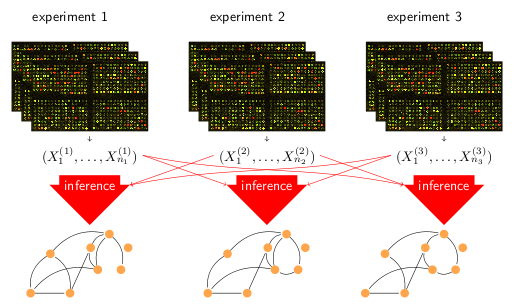
\epsfig{file=\fignet/multitask.eps, clip=, width=0.6\textwidth} 
      \end{tabular}
    \end{tabular}
  }

%==================================================================== 
\subsection{Non regularized methods}
\frame{ \frametitle{Efficient algorithm for network learning}
%==================================================================== 

  \paragraph{GGM.} Alternatives to convex optimization techniques can be used for network inference. \refer{GHV12} propose both an algorithm with statistical guaranties in terms of model selection.
  
  \bigskip \bigskip \Pause
  \paragraph{Bayesian networks} provide a larger framework than GGM but do not benefit from nice Gaussian properties and associated algorithms. \\ ~ \\
  \ra Efficient heuristics are needed to explore the (huge) space of graphs.
  \refer{VVA12}, \refer{VMG12}
  
  \bigskip \bigskip 
  \paragraph{Update:} \Refer{Champion and al. (poster)},  \Refer{Schwaller (next talk)}

}


%==================================================================== 
\subsection{Detection limit}
\frame{ \frametitle{Detection limit}
%==================================================================== 

%  The 'large $p$, small $n$' paradigm raises serious theoretical statistical issues. \\
  
%   Network inference in the GGM context is related to regression: e.g. finding which genes (with expression $\bf X$) control the expression of a given gene (denoted $Y$).

%  \bigskip \Pause   
  \paragraph{Regression context.} Consider a network with $p$ genes, $n$ replicates. 
  
  \bigskip 
  {Detection limits in Gaussian regression models}  vary with the problem: \Pause 
  \begin{enumerate}
   \item Prediction %of the expression of the target gene
%    {\color{black} Estimating a signal} $\mathbb{E}[{\bf Y}]={\bf }\theta$.~\\
%   {\bf $\neq $} prediction in a {\color{black} random design} setting: Estimate $\mathbb{E}[Y_{\text{new}}|X_{\text{new}}]$.
   \item Testing if the target gene is regulated: \\
%   ${\bf H_0}$= '{\color{black} $\theta=0$}' vs  ${\bf H_1}$= '$\theta\neq 0$ but $\theta$ is sparse in some sense'.
   \item Estimating the coefficients (inverse problem).
   \item Recovering the set of parent genes (support estimation).
   \item Estimating a set that contain the support (dimension reduction).
   \end{enumerate}
   
   \Pause \bigskip
   \refer{Ver12} shows that a transition phase in terms of minimax risk is observed between
   $$
   k \log \frac{p}k \leq n \qquad \text{and} \qquad k \log \frac{p}k > n \log n
   $$
   where $k = $size of the support.
 }
 
  
%==================================================================== 
\subsection{Testing edges}
\frame{ \frametitle{Testing edges}
%==================================================================== 

  More specific question: Should a specific edge be added to a preliminary network?
  $$
  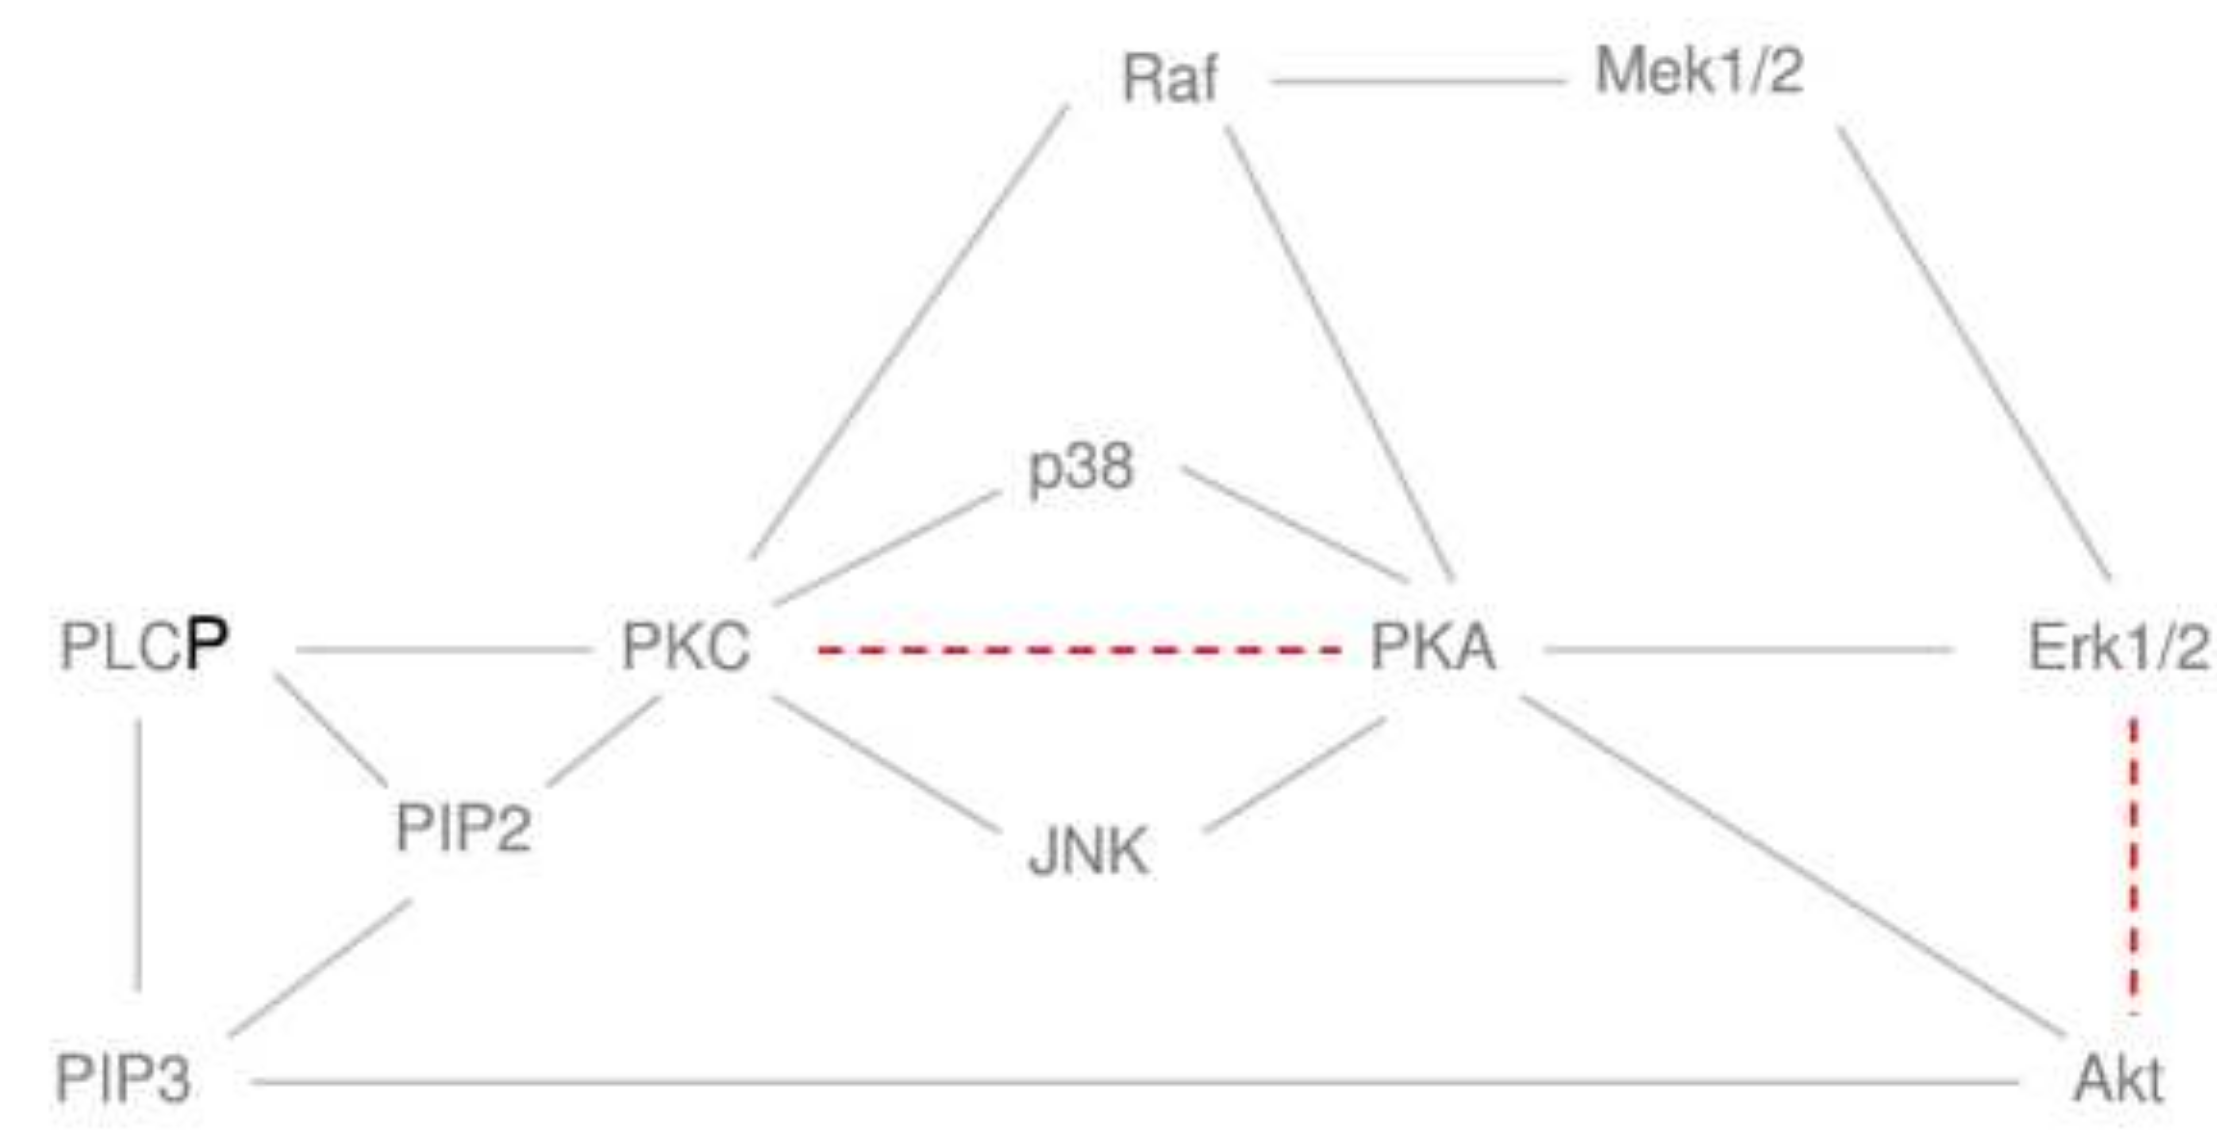
\epsfig{file=\fignet/Sac05-Fig.eps, clip=, width=0.6\textwidth} 
  $$
  
  Multiple testing issues arise. \refer{VeV09} provide a procedure with control of the level and guaranty as for the power. (see also \refer{VSB08})

}

%====================================================================
%====================================================================
\section{Network structure}
\frame{ \frametitle{Network structure}}
%====================================================================

%====================================================================
\frame{ \frametitle{Network structure: General framework}
%====================================================================

  \paragraph{Network structure.} How to get a global picture of the global organization of a large observed graph (with thousands or more node)
  
  \bigskip \bigskip \Pause
  \paragraph{Probabilistic models.} Most of our contributions rely on 
  \begin{itemize} 
   \item some probabilistic modeling of the observed network
   \item involving some hidden (or latent) structure.
  \end{itemize}
  
  \bigskip \bigskip \Pause
  \paragraph{What for?}
  \begin{itemize}
  \item To be able to better understand networks' structures,
  \item To be able to simulate 'realistic' networks,
  \item To retrieve underlying structures.
  \end{itemize}

}

%====================================================================
\subsection{Random graph models}
%====================================================================

%====================================================================
\frame{ \frametitle{Scale-free model based on bipartite graphs} 

  \bigskip \bigskip
  \textcolor{gray}{
  \paragraph{Topogical specificities.} Many biological networks, display 'scale-free' degree distribution, 'small world' structure and contain a giant component.}

  \bigskip 
  \textcolor{gray}{
  Such characteristics can derive from a simple random graph model, involving a hidden layer. \refer{Bir09a}}

  \bigskip\bigskip
  \begin{tabular}{cc}
    \hspace{-.5cm}
    \begin{tabular}{p{.4\textwidth}}
      \textcolor{gray}{
        \paragraph{Bipartite graph.} 2 categories of nodes exist.} \\ 
        \smallskip
      \textcolor{gray}{
        \paragraph{Projected graph.} We observe only the projection of the complete graph on one category.}
        \vspace{3cm}~ 
    \end{tabular}
    & 
    \hspace{-.75cm}
    \begin{tabular}{p{.55\textwidth}}
        \epsfig{file=\fignet/Bipartite-Proj.eps, width=.65\textwidth, clip=} 
    \end{tabular}
  \end{tabular}

}

%====================================================================
\frame{ \frametitle{Stochastic block-model (SBM) for interaction graphs} 

  \paragraph{Heterogeneity.} Biological networks display heterogeneous structures (hubs, modularity, \dots).

  \bigskip \bigskip \Pause
  \paragraph{Hidden structure.} To account for some heterogeneity, assume 
  \begin{itemize}
  \item that each node has some hidden (unknown) characteristics
  \item and that connections between nodes depend on their
    characteristics.
  \end{itemize}

  \bigskip \Pause
  \begin{tabular}{cc}
    \hspace{-.5cm}
    \begin{tabular}{p{.5\textwidth}}
      \paragraph{Stochastic Block-Model (SBM):} \\
      A simple random graph model:
      \begin{itemize}
      \item A label $Z_i \in \{1, \dots K\}$ is associated with each node $i$;
      \item The connexion probability between node $i$ and $j$ depends on both
      $Z_i$ and $Z_j$.
      \end{itemize}
      \\~ \\~ \\~ \\~
    \end{tabular}
    & 
    \hspace{-.5cm}
    \begin{tabular}{p{.5\textwidth}}
            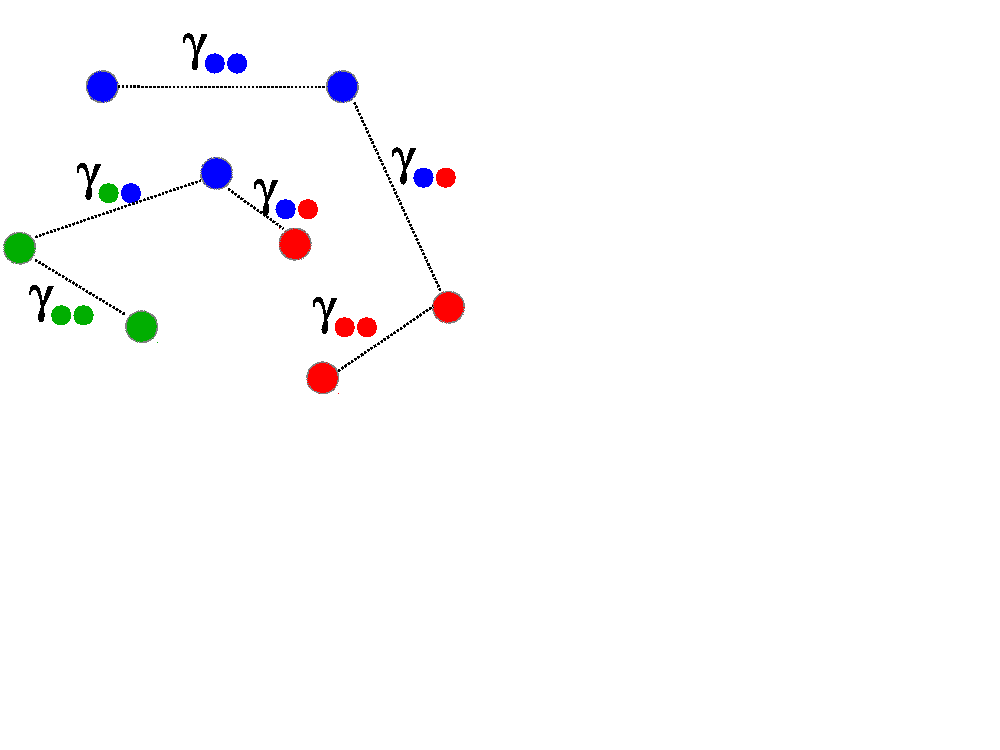
\epsfig{file = \fignet/FigSBM-Model-3.eps,
          width=.75\textwidth, clip=}    
    \end{tabular}
  \end{tabular}
  
  
}

% %====================================================================
% \frame{ \frametitle{Stochastic block-model for interaction graphs} 
% 
%   \paragraph{Heterogeneity.} Many biological networks display
%   heterogeneous structures (hubs, highly-connected subsets,
%   modularity, \dots) that can not be explained by simple random graph
%   models.
% 
%   \bigskip \Pause
%   \paragraph{Hidden structure.} A standard way to account for such an
%   heterogeneity is to assume 
%   \begin{itemize}
%   \item that each node has some hidden (unknown) characteristics
%   \item and that connections between nodes depend on their
%     characteristics.
%   \end{itemize}
% 
%   \bigskip \Pause
%   \paragraph{Stochastic Block-Model (SBM)} A simple random graph model:
%   \begin{itemize}
%   \item Nodes $i = 1\dots n$ are spread into $K$ groups with proportions
%     \emphase{$\alpha_1, \dots \alpha_K$},
%   \item \emphase{$Z_i$} denotes the \emphase{unobserved label} of node $i$,
%   \item \emphase{$X_{ij}$} denotes the presence of an edge between
%     nodes $i$ and $j$ 
%   \end{itemize}
%   $$
%   \emphase{\pi_{k\ell}} = \Pr\{X_{ij} = 1 | Z_i=k, Z_j = \ell\}.
%   $$
% }

%====================================================================
\subsection{Inference of SBM}
%====================================================================

%====================================================================
\frame{ \frametitle{SBM: A typical case of intractable distribution ...}

  \begin{tabular}{cc}
    \hspace{-.5cm}
    \begin{tabular}{p{.5\textwidth}}
      \onslide+<1->{
        \paragraph{Maximum likelihood.} MLE of $\thetabf$ 
        obtained via the E-M algorithm ... \\
        provided that we can calculate
        $$
        P(\Zbf | \Xbf; \thetabf).
        $$
        ~\\~\\~\\
      }
    \end{tabular}
    & 
    \hspace{-.5cm}
    \begin{tabular}{p{.5\textwidth}}
            \begin{overprint}
        \onslide<2>
        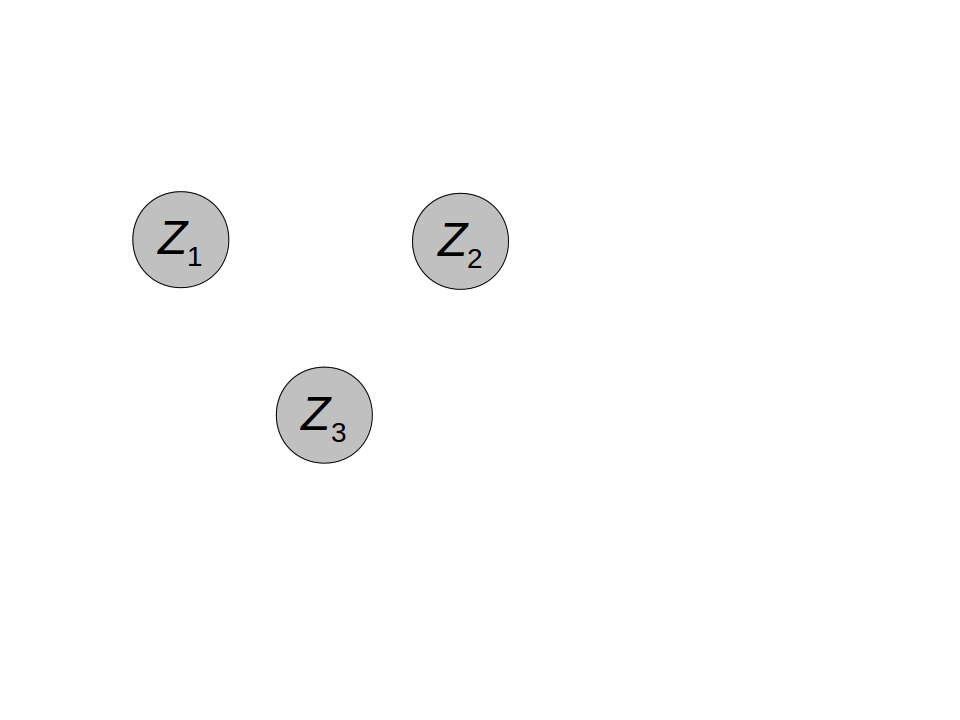
\epsfig{file=../FIGURES/FigSBM-Z.eps, clip=, width=0.6\textwidth}
        \onslide<3>
        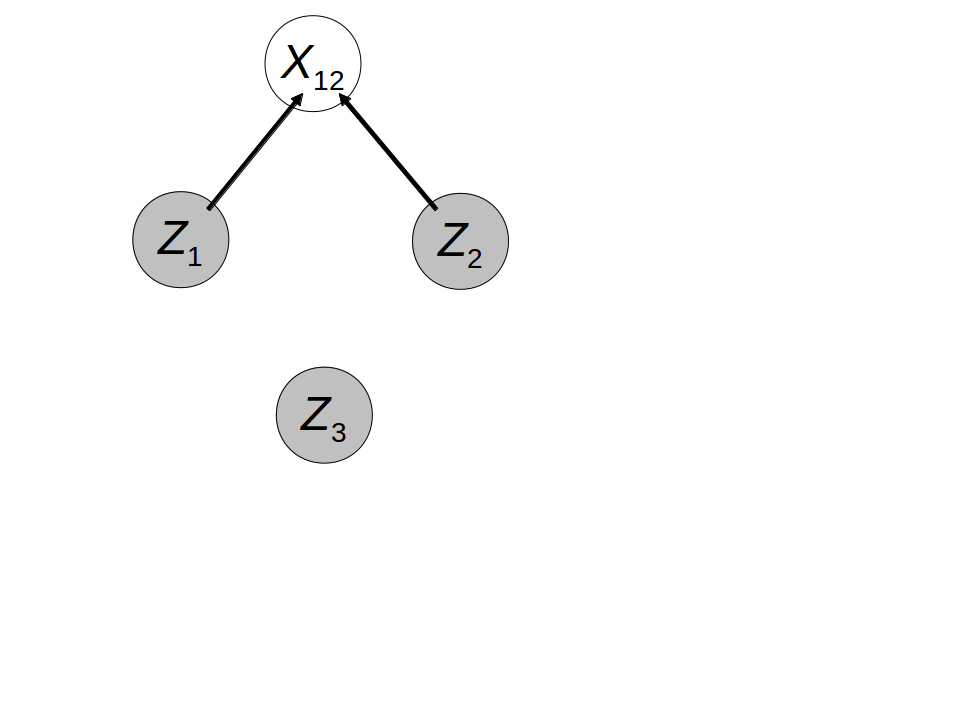
\epsfig{file=../FIGURES/FigSBM-Z-X12.eps, clip=, width=0.6\textwidth}
        \onslide<4>
        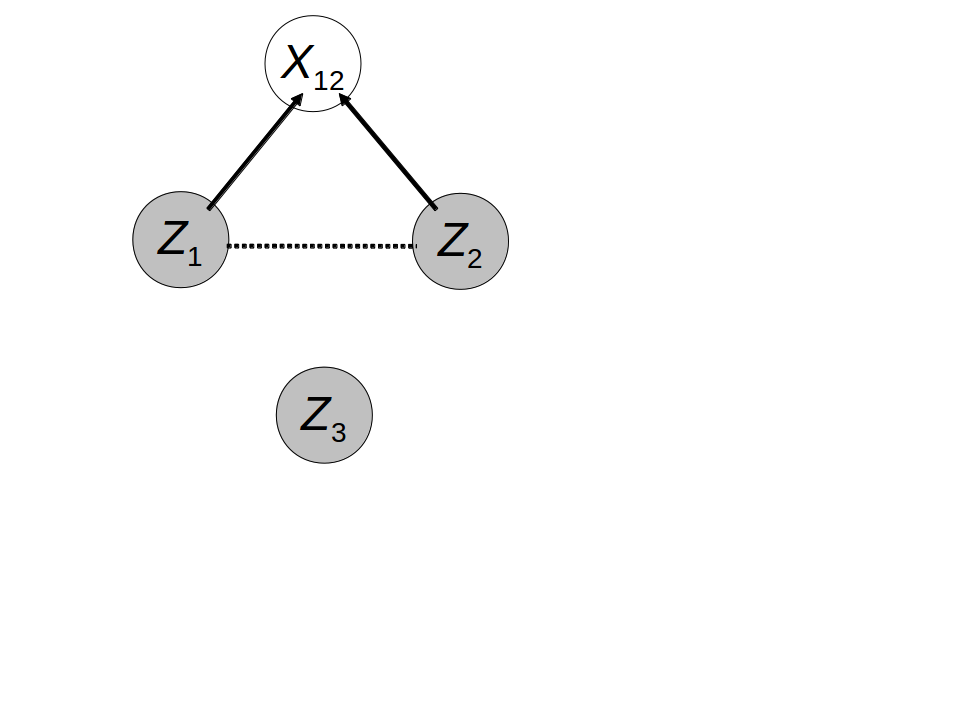
\epsfig{file=../FIGURES/FigSBM-Z-X12-Moral.eps, clip=,
          width=0.6\textwidth} 
        \onslide<5>
        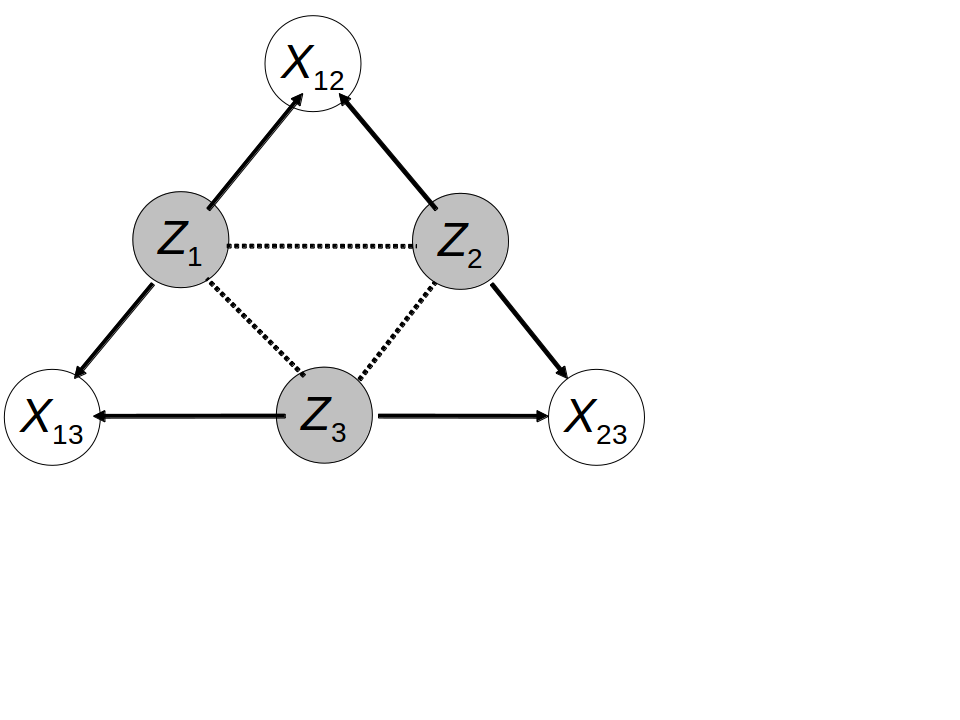
\epsfig{file=../FIGURES/FigSBM-Z-X-Moral.eps, clip=,
          width=0.6\textwidth} 
        \onslide<6->
        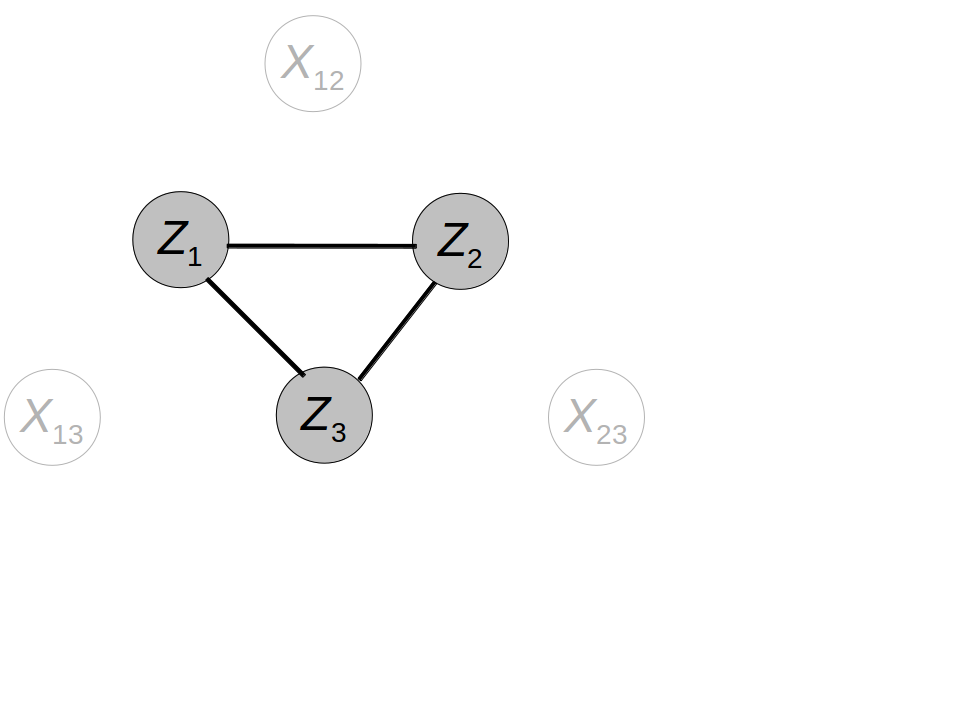
\epsfig{file=../FIGURES/FigSBM-ZcondX.eps, clip=,
          width=0.6\textwidth}
      \end{overprint}
    \end{tabular}
  \end{tabular}

  \onslide+<6->{
    \vspace{-1.5cm}
    \paragraph{Conditional distribution.} The dependency graph of
    $\Zbf$ given $\Xbf$ is a clique. \\
    \ra No factorization can be hoped (unlike for HMM or other tree models). \\
    \ra $P(\Zbf | \Xbf; \thetabf)$ can not be computed
    (efficiently). \\
    \ra Variational techniques provide 
    $$
    Q(\Zbf) \simeq P(\Zbf | \Xbf)
    $$
    using, e.g., a mean-field approximation.
  }
}

%====================================================================
\frame{\frametitle{Getting worth in a Bayesian setting}
  
  \begin{tabular}{cc}
    \hspace{-.5cm}
    \begin{tabular}{p{.5\textwidth}}
% 	 \vspace{-2cm}
      We are now interested in 
      $$
      P(\Zbf, \thetabf | \Xbf).
      $$
      ... More intricate than $P(\Zbf | \Xbf; , \thetabf)$.

      \onslide+<4->{
	 \vspace{.5cm}
	 \paragraph{Variational problem:} find \\
	 ~\\ ~\\ 
	 }	
    \end{tabular}
    & 
    \hspace{-.5cm}
    \begin{tabular}{p{.5\textwidth}}
      \begin{overprint}
        \onslide<2>
        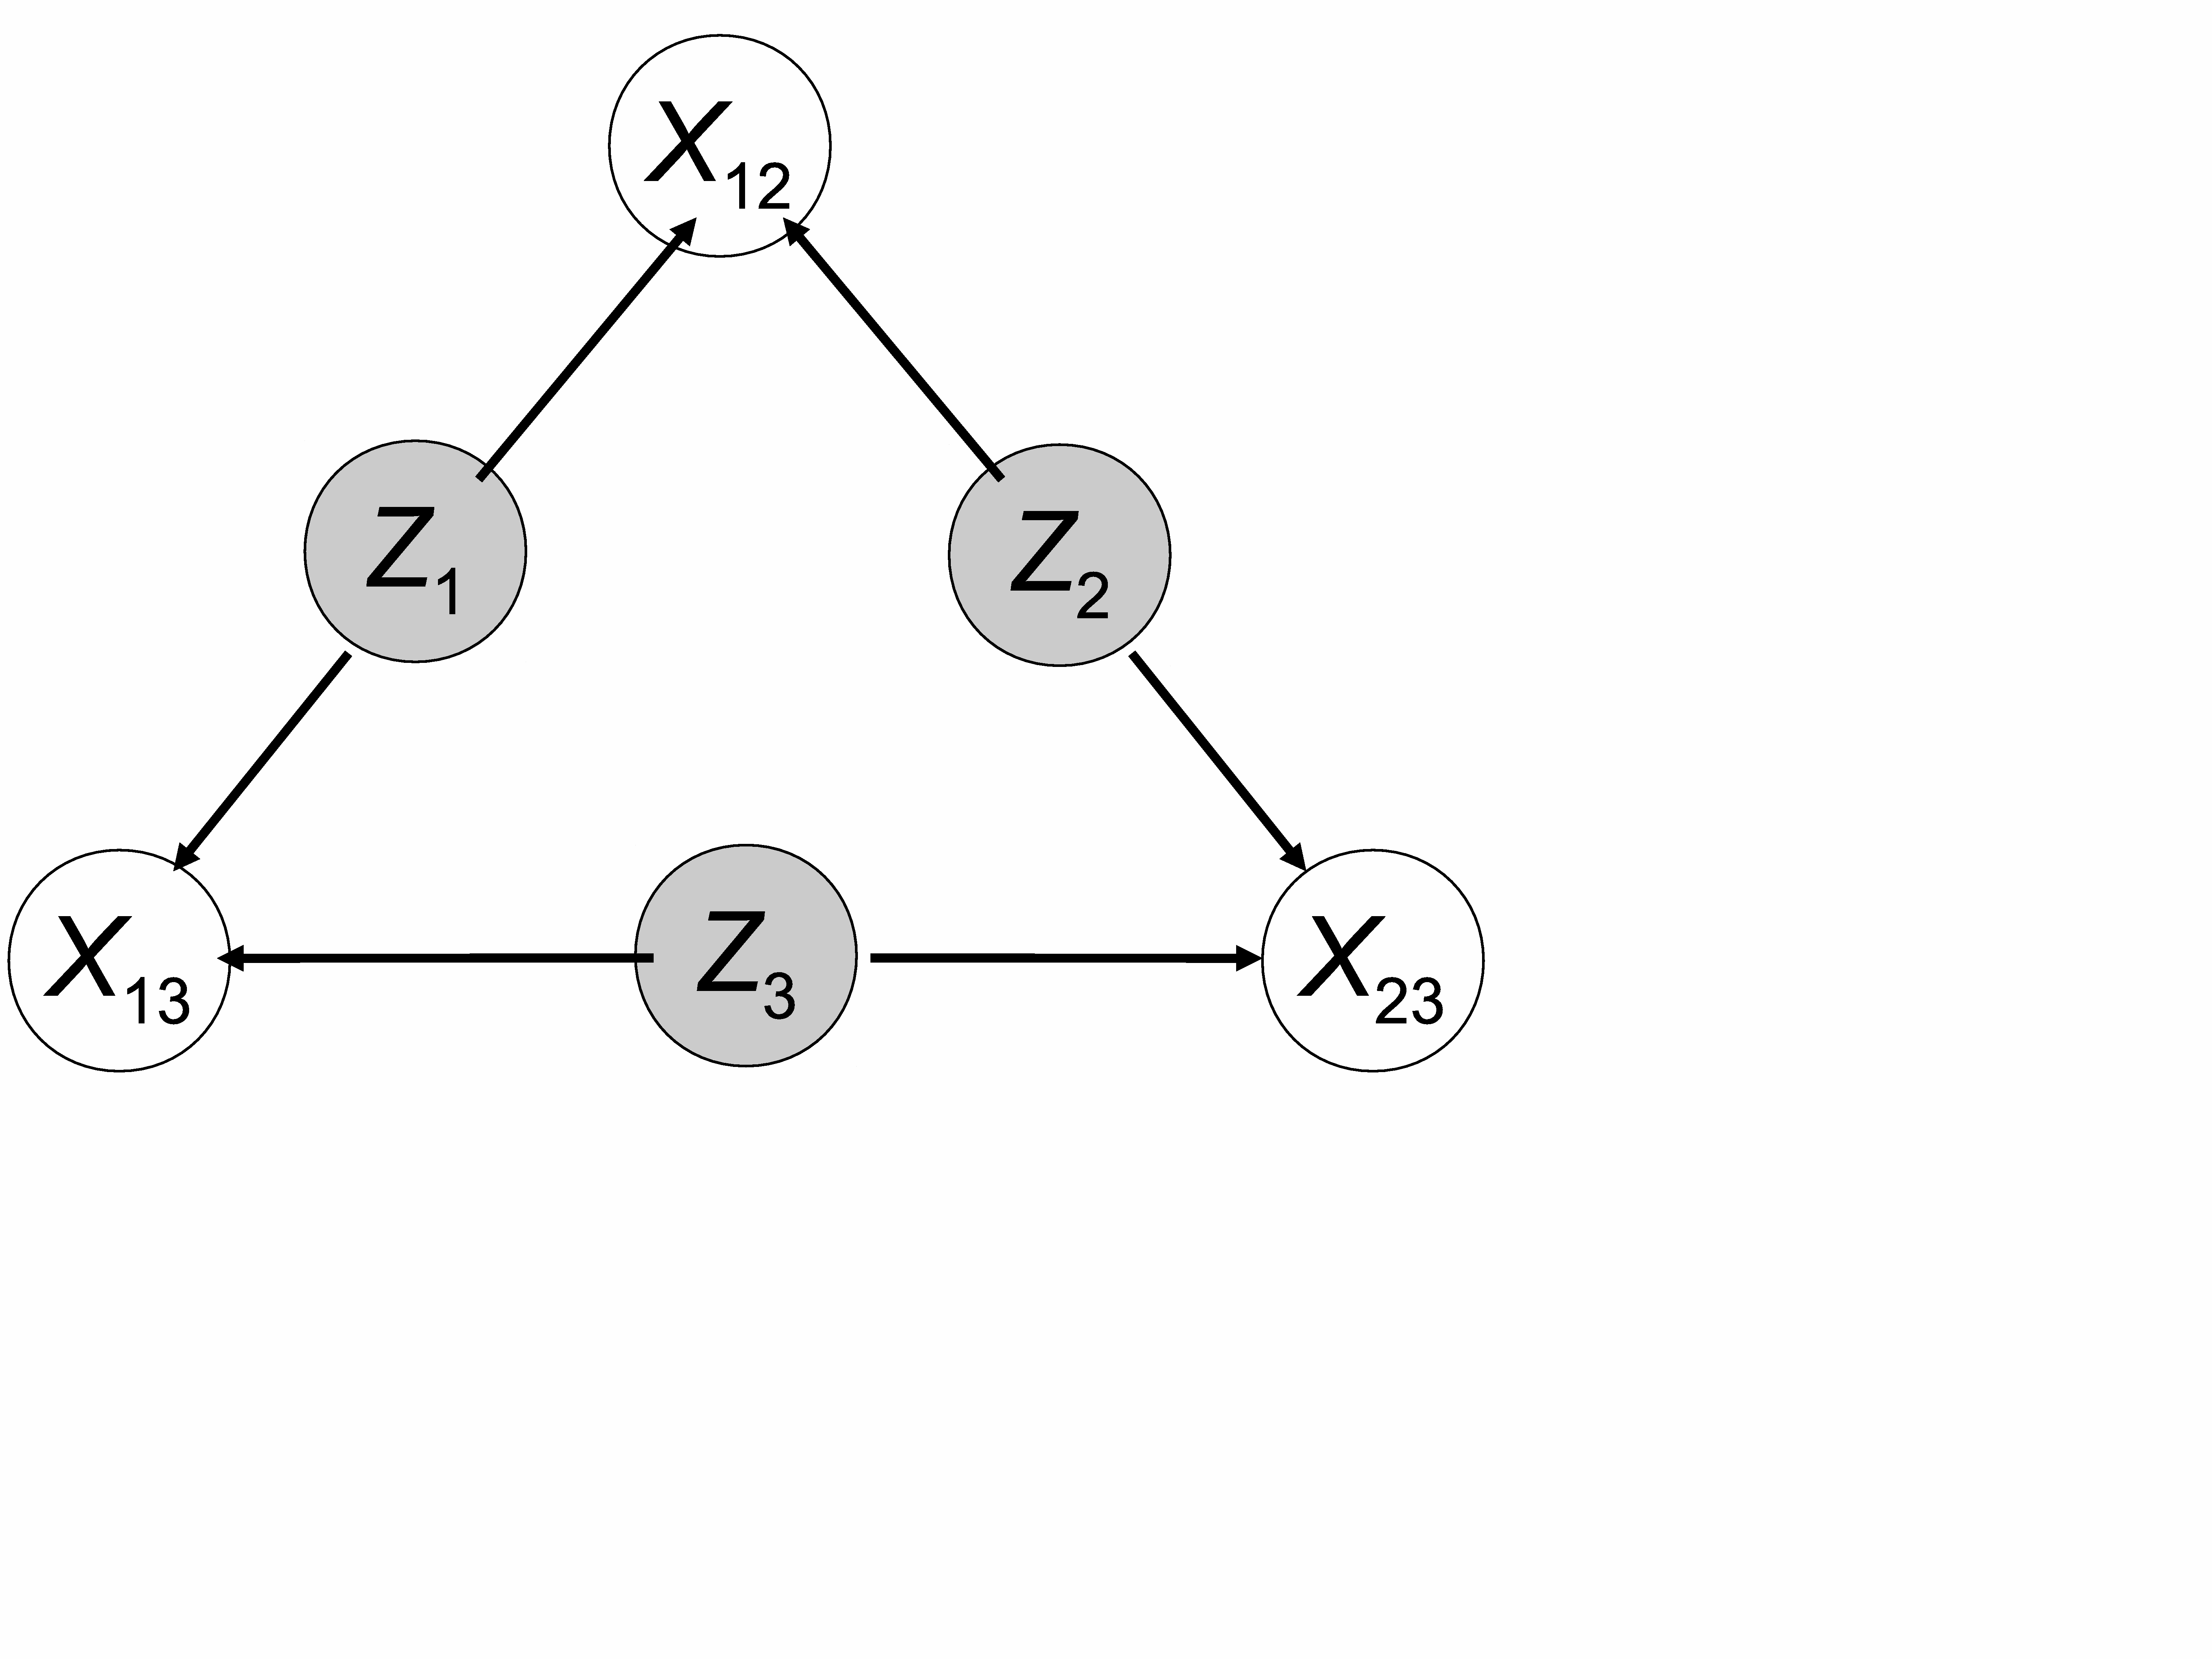
\epsfig{file = \fignet/FigSBM-Z-X.eps,
          width=.7\textwidth, clip=}   
        \onslide<3>
        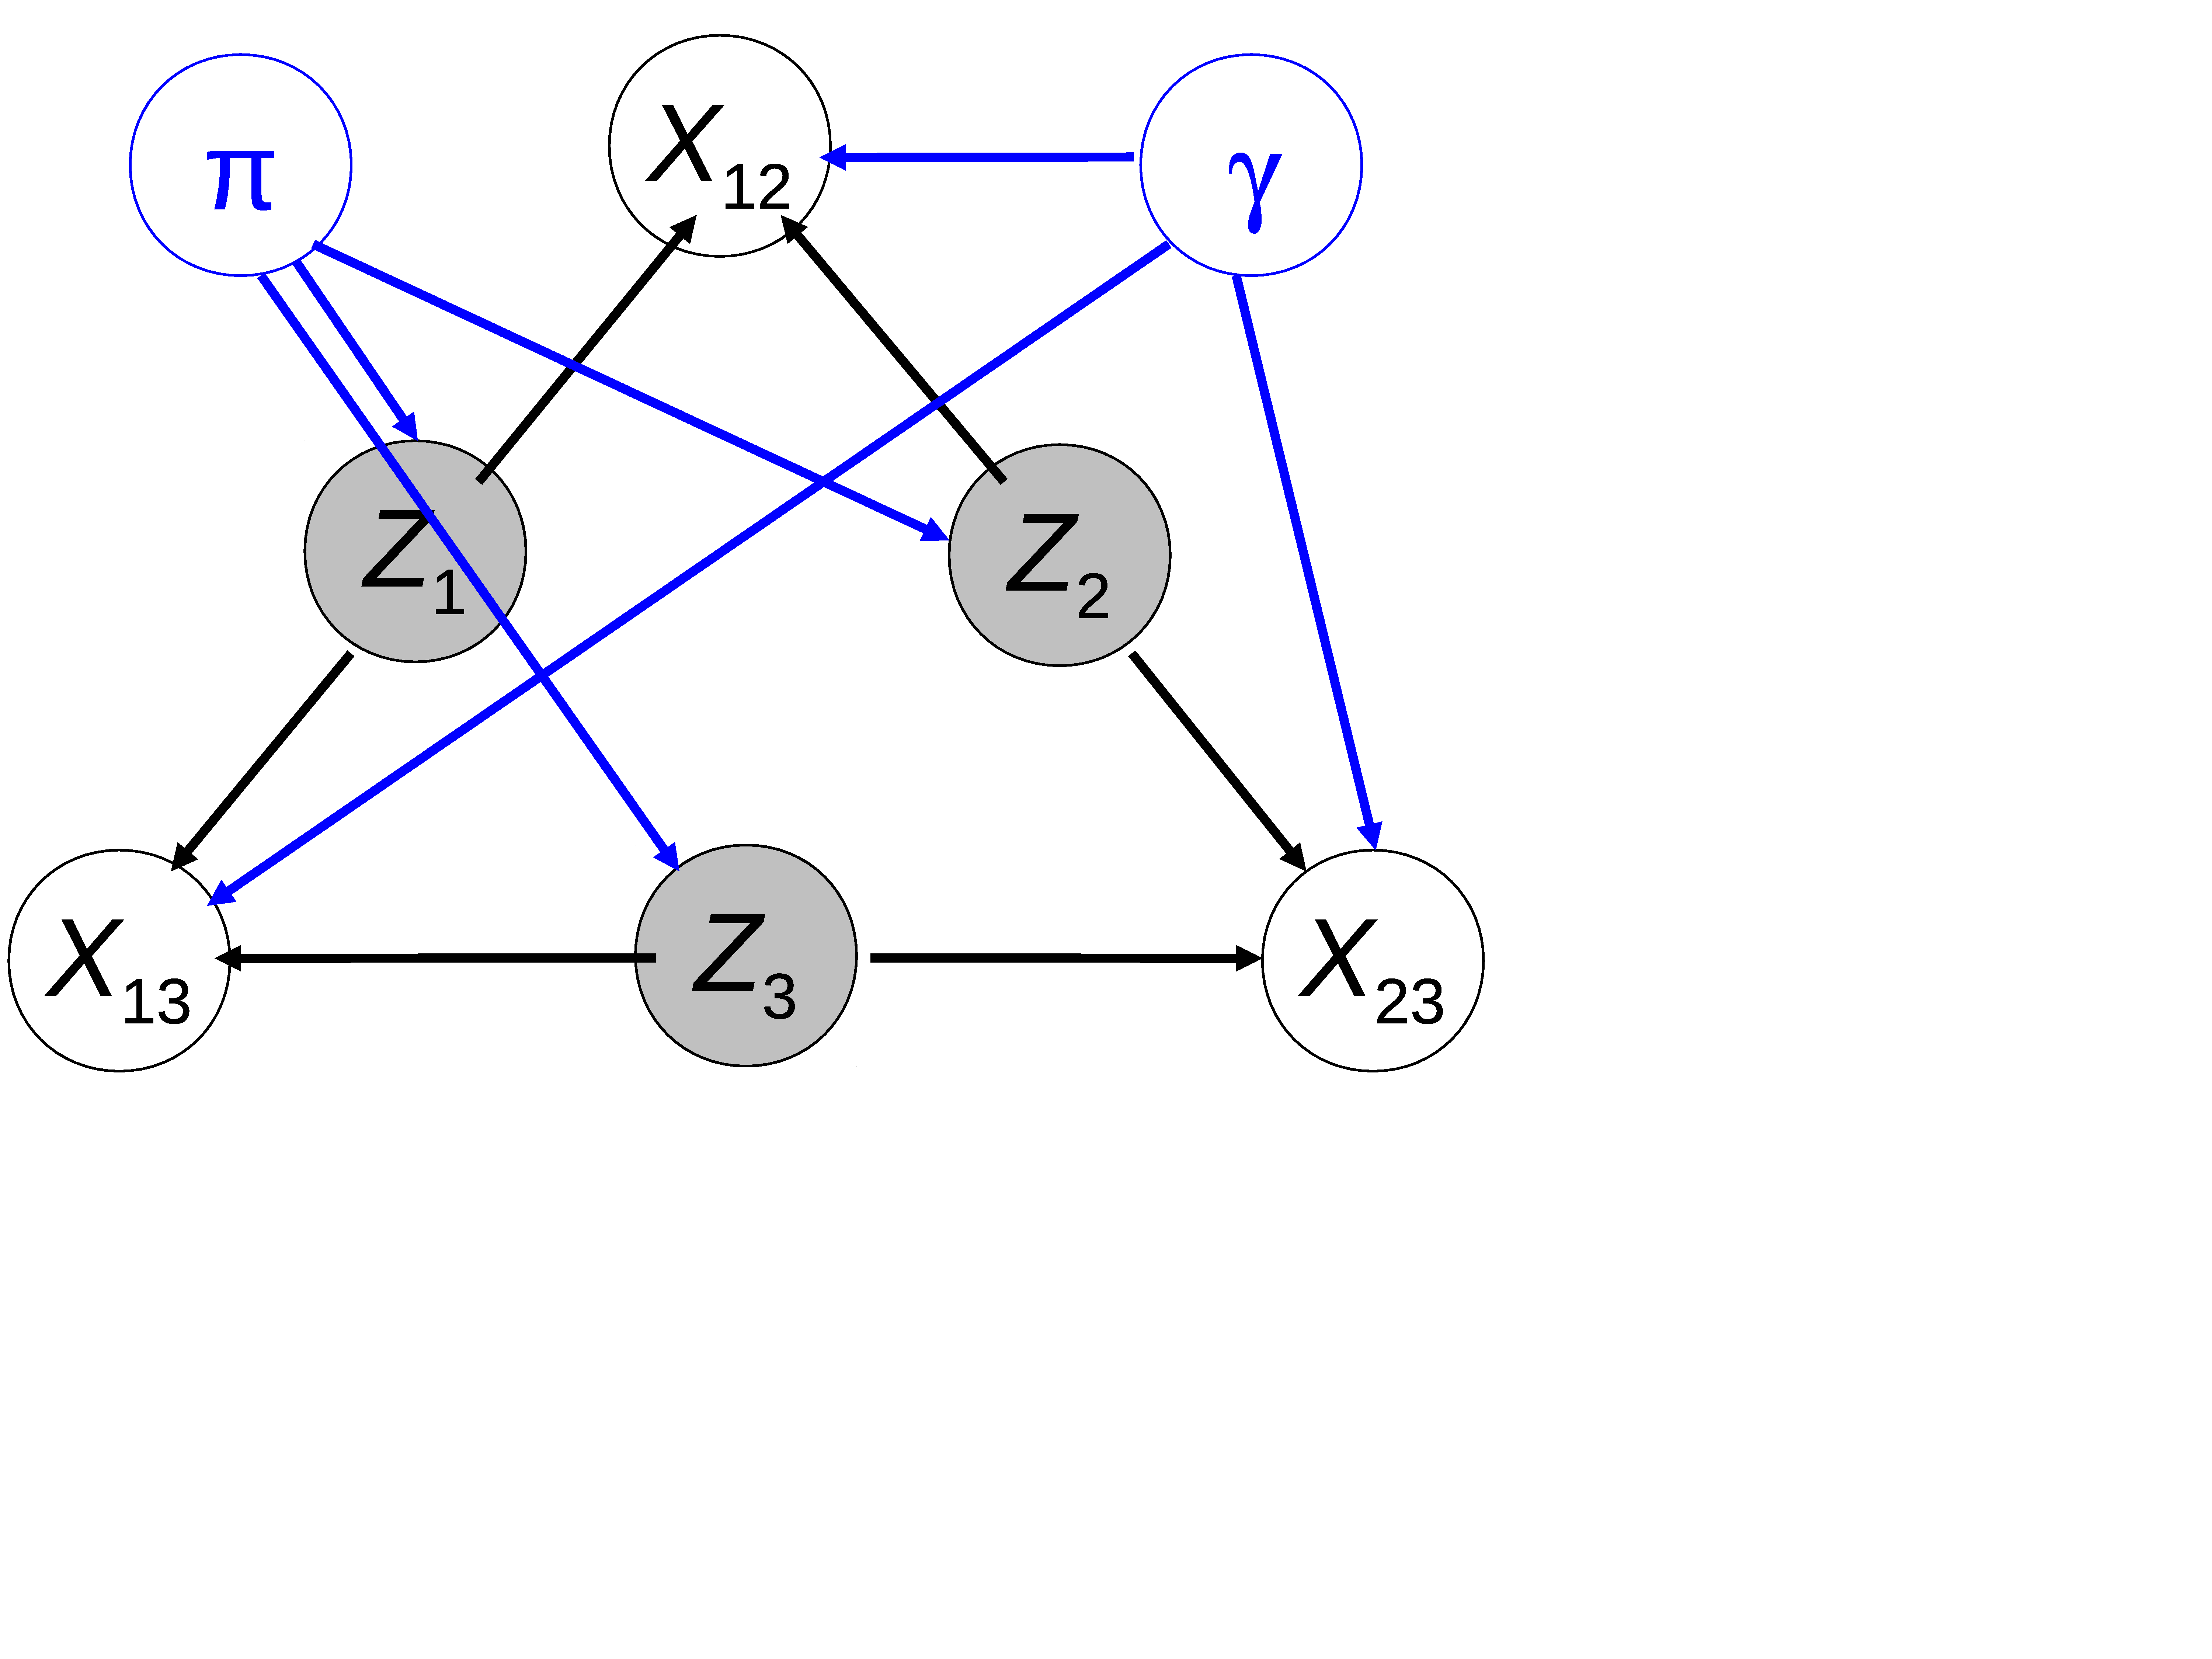
\epsfig{file = \fignet/FigSBM-Bayes-1.eps,
          width=.7\textwidth, clip=}   
        \onslide<4->
        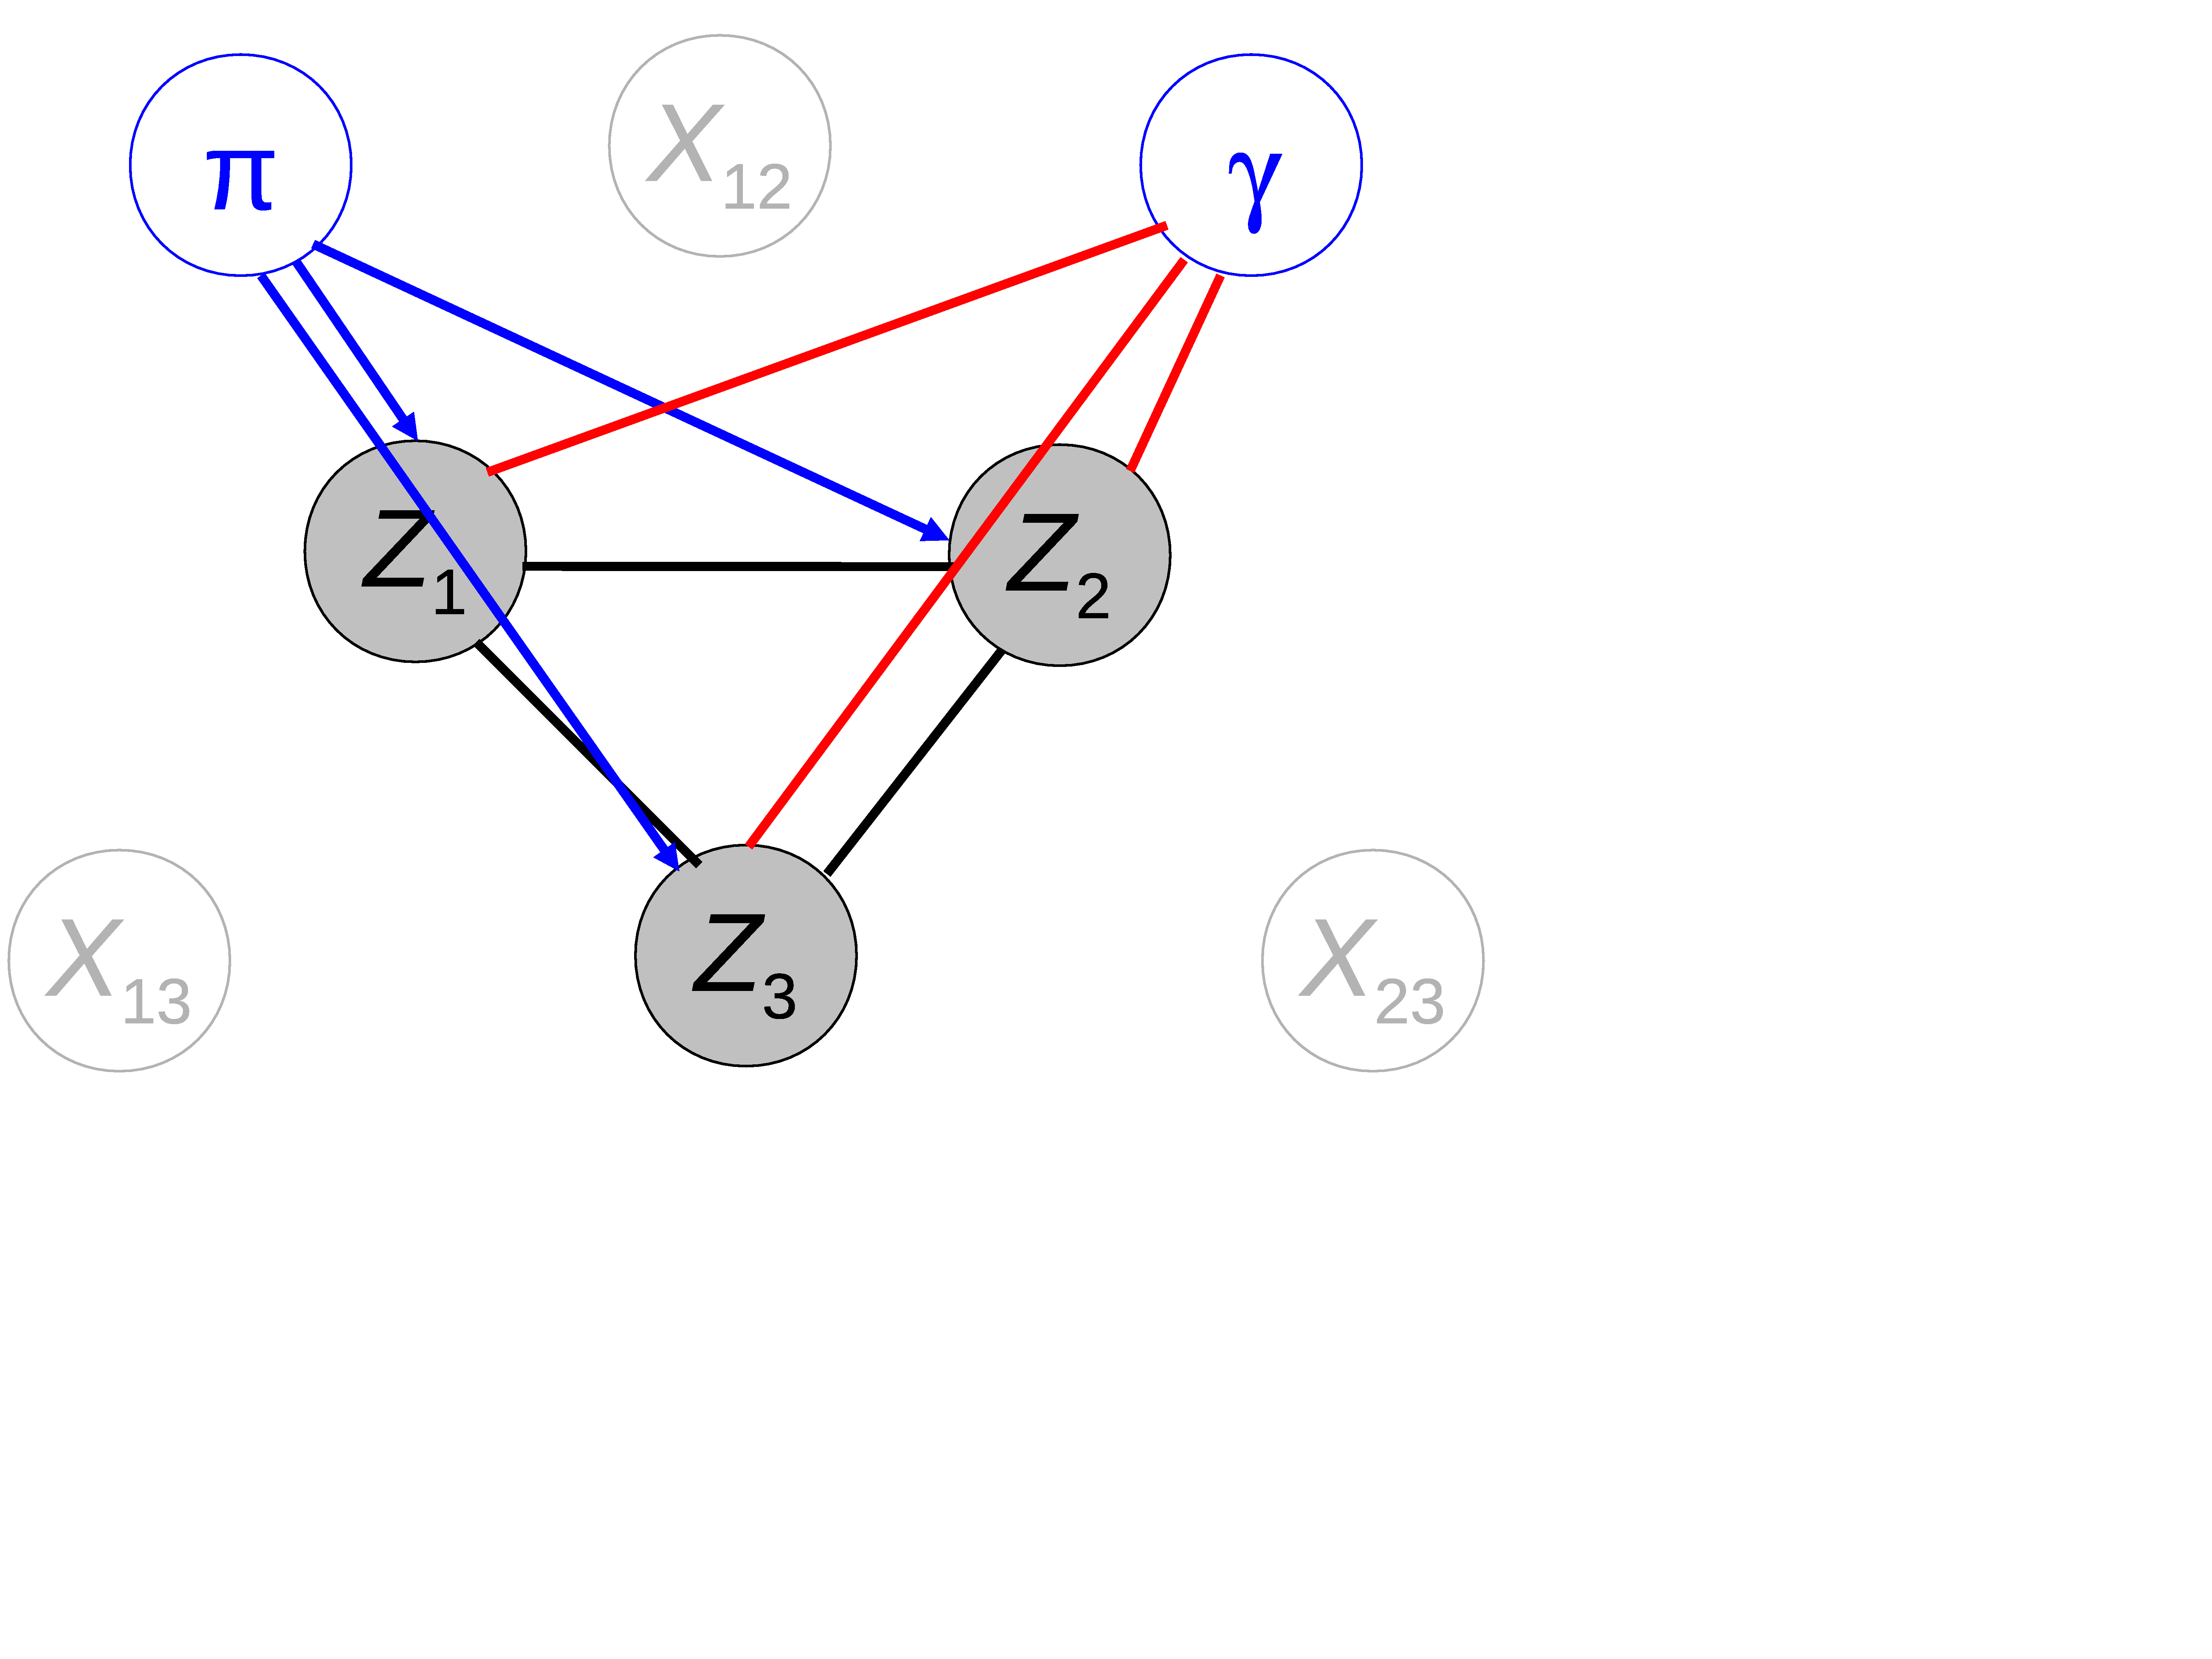
\epsfig{file = \fignet/FigSBM-Bayes-2.eps,
          width=.7\textwidth, clip=}   
      \end{overprint}
    \end{tabular}
  \end{tabular}
  
  \onslide+<4->{
    \vspace{-2.5cm}
    $$
    Q^*(\Zbf, \thetabf) = \underset{Q \in \Qcal}{\arg\min} KL(Q(\Zbf, \thetabf) || P(\Zbf, \thetabf | \Xbf)).
    $$
    }
    
  \onslide+<5>{\bigskip
  \paragraph{Variational Bayes EM:} 
  Taking $\Qcal = \{Q: Q = Q_{\Zbf} Q_{\thetabf}\}$,
  gives
  $$
  Q^*_{\Zbf}(\Zbf) \propto \exp \left[\Esp_{Q^*_{\thetabf}} \log P(\Xbf, \Zbf, \thetabf) \right], \quad
  Q^*_{\thetabf}(\thetabf) \propto \exp \left[\Esp_{Q^*_{\Zbf}} \log P(\Xbf, \Zbf, \thetabf) \right].
  $$
%   \begin{eqnarray*}
%    Q^*_{\Zbf}(\Zbf) & \propto & \exp \left[\Esp_{Q^*_{\thetabf}} \log P(\Xbf, \Zbf, \thetabf) \right] \\
%    Q^*_{\thetabf}(\thetabf) & \propto & \exp \left[\Esp_{Q^*_{\Zbf}} \log P(\Xbf, \Zbf, \thetabf) \right].
%   \end{eqnarray*}
  }

  }

%-------------------------------------------------------------------- 
\frame{ \frametitle{SBM analysis of {\sl E. coli} operon networks}

  \vspace{-0.5cm}
  \hspace{-0.5cm}
  \begin{tabular}{cc}         
    \begin{tabular}{p{0.45\textwidth}}
%       \onslide+<1->{
	%\vspace{-1cm}
        \epsfig{file=\fignet/im_EcoliVEM_2.ps,
          width=.45\textwidth, clip=} \\
          %~\\
          \refer{PMD09}
%         }
    \end{tabular}
    &
    \begin{tabular}{p{0.45\textwidth}}
%     \onslide+<2->{
      %\vspace{-.3cm}
      \paragraph{Meta-graph representation.} \\
      %\vspace{-.5cm}
      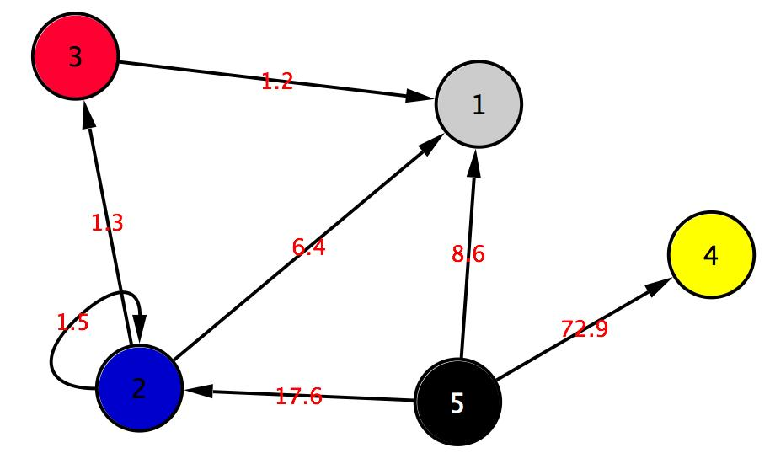
\epsfig{file=\fignet/VEMmetagraphe.ps,
      width=.35\textwidth, clip=}  \\
%     }
%     \onslide+<3->{
      \vspace{-.3cm}
      \paragraph{Parameter estimates.} $K = 5$     \\
      \includegraphics[width=.35\textwidth]{../FIGURES/im-pi1BVEM}\\        
      \includegraphics[width=.35\textwidth]{../FIGURES/im-pi2BVEM}\\
      \includegraphics[width=.35\textwidth]{../FIGURES/im-pi3BVEM}\\
      \includegraphics[width=.35\textwidth]{../FIGURES/im-pi4BVEM}\\
      \includegraphics[width=.35\textwidth]{../FIGURES/im-pi5BVEM}\\
      \hline 
      \includegraphics[width=.35\textwidth]{../FIGURES/im-alphaBVEM}\\
%     }
    \end{tabular}
  \end{tabular}
  }

%====================================================================
\frame{ \frametitle{Inference of SBM: A lot of statistical issues (1/2)}

  \paragraph{Identibiability of SBM.} \refer{AMR09}

  \bigskip \bigskip \Pause
  \paragraph{Variational inference.} Including the choice of $K$:
  \begin{itemize}
  \item frequentist version (variational EM) \refer{DPR08}
  \item bayesian version (variational Bayes) \refer{LBA11b}
  \end{itemize}

  \bigskip \bigskip \Pause
  \paragraph{Understanding variational inference.} As it is an approximation we had to
  \begin{itemize}
  \item see if it works \refer{GDR11}
  \item understand why it works \refer{CDP12}
  \end{itemize}
  
  \bigskip 
  \paragraph{Update:} \refer{MaM14}
}
%====================================================================
\frame{ \frametitle{Inference of SBM: A lot of statistical issues (2/2)}

  \paragraph{Alternative inference strategies:} To scale with large networks
  \begin{itemize}
  \item pseudo-likelihood estimator: \refer{AmM09}
  \item linear time estimator based on the degrees: \refer{CDR12}
  \end{itemize}

  \bigskip \bigskip \Pause
  \paragraph{Generalizations of SBM.} Extend the SBM framework
  \begin{itemize}
  \item to continuous latent space \refer{DPV10}
  \item to account for covariates (with weighted edges) \refer{MRV10}
  \item to overlapping classes \refer{LBA11a}
  \end{itemize}

  \bigskip \bigskip 
  \paragraph{Update:} \refer{LVD13} \\
  + on ArXiv: \Refer{Latouche and R. (2013)}\nocite{LaR14}, \Refer{Matias and R. (2014)}\nocite{MaR14}, \refer{ArV13}
  
}

%====================================================================
%====================================================================
\section{Network Motifs}
\frame{ \frametitle{Network Motifs} }
%====================================================================


%====================================================================
%====================================================================
\section{Tools \& Workshop}
\frame{ \frametitle{Tools \& Workshops}
%====================================================================

  \begin{tabular}{cc}
    \hspace{-.5cm}
    \begin{tabular}{p{.5\textwidth}}
      \paragraph{Packages.}
      \begin{itemize}
      \item \paragraph{Simone.} Regularization-based network inference
      \item \paragraph{GGMselect.} Model selection for network inference. 
      \item \paragraph{GeneBayesNet.} Bayesian network \refer{VMV12} %\\~
      \item \paragraph{MixNet. } Stochastic block-model inference
      \item \paragraph{Mixer. } Stochastic block-model (+ extensions)
      \item \paragraph{WMixNet. } Weighted SBM \refer{Leg14} %\\~
      \item \paragraph{NeMo. } Counting and assessing exceptional network motifs
      \item \paragraph{Paloma. } Locally exceptional motif \refer{Bir12}
      \end{itemize}
    \end{tabular}
    & 
    \hspace{-.5cm} \Pause
    \begin{tabular}{p{.45\textwidth}}
      \paragraph{MIA working groups (networks).} 
      \begin{itemize}
      \item SSBnet: subgroup of SSB \\~
      \item AIGM: Approximate inference in graphical models \\~
      \item NetBio : Biological networks \\~
      \item SonataStat : A. thaliana gene network inference \\~
      \end{itemize}
      ~\\
      \paragraph{MIA support for workshop.} 
      \begin{itemize}
      \item SMPGD: yearly meeting on statistics for genomics
      \end{itemize}
    \end{tabular}
  \end{tabular}
}

%====================================================================
{\tiny
  \bibliography{/home/robin/Biblio/ARC,/home/robin/Biblio/AST,
    /home/robin/Biblio/SSB} 
  \bibliographystyle{/home/robin/LATEX/Biblio/astats}
  %\bibliographystyle{plain}
  }
%====================================================================

\appendix

%====================================================================
\section{Network Motifs}
\frame{ \frametitle{Network Motifs} 
%====================================================================

\paragraph{Motifs = Local patterns} that constitute {functional modules}
  or basic building blocks of complex networks.
  \begin{itemize}
  \item \paragraph{Transcription regulatory networks:} 
    motifs may perform specific regulatory functions
    (e.g. feed-forward loop, bi-fan).
  \item \paragraph{Metabolic motif} may reveal systematic associations of
    reactions in metabolic pathways. 
  \end{itemize}

  \bigskip\Pause
  \paragraph{Motif detection.} To detect 'exceptional motifs', we need
  to
  \begin{enumerate}
  \item Give a precise (topological) definition of a motif $\mbf$;
  \item Be able to count (efficiently) motif occurrences in a given
    network;
  \item Define a random graph model as a null model $G_0$;
  \item Know the (approximate) distribution of the number occurrences
    under the null model to assess the significance with a $p$-value.
  \end{enumerate}

  }

%==================================================================== 
\subsection{Motif definition}
%====================================================================
\frame{\frametitle{Different motifs for different networks}
  \begin{tabular}{cc}
    \hspace{-.5cm}
    \begin{tabular}{p{.45\textwidth}}
      \paragraph{Metabolic networks.} Colored \\graph
      \begin{itemize}
      \item Nodes = reactions
      \item Color = type
      \item Edges = shared compound
      \end{itemize}
    \end{tabular}
    & 
    \hspace{-.5cm}
    \begin{tabular}{p{.45\textwidth}}
      \paragraph{Interaction networks.} (Oriented) graph
      \begin{itemize}
      \item Nodes = proteins, genes
      \item Edges = interactions, regulations
      \end{itemize}
    \end{tabular}
  \end{tabular}

  \Pause
  \begin{tabular}{cc}
    \hspace{-.5cm}
    \begin{tabular}{p{.45\textwidth}}
      \paragraph{Motif.} Connected component with prescribed color
      frequency
      \begin{center}%$$
        \vspace{-.5cm}
        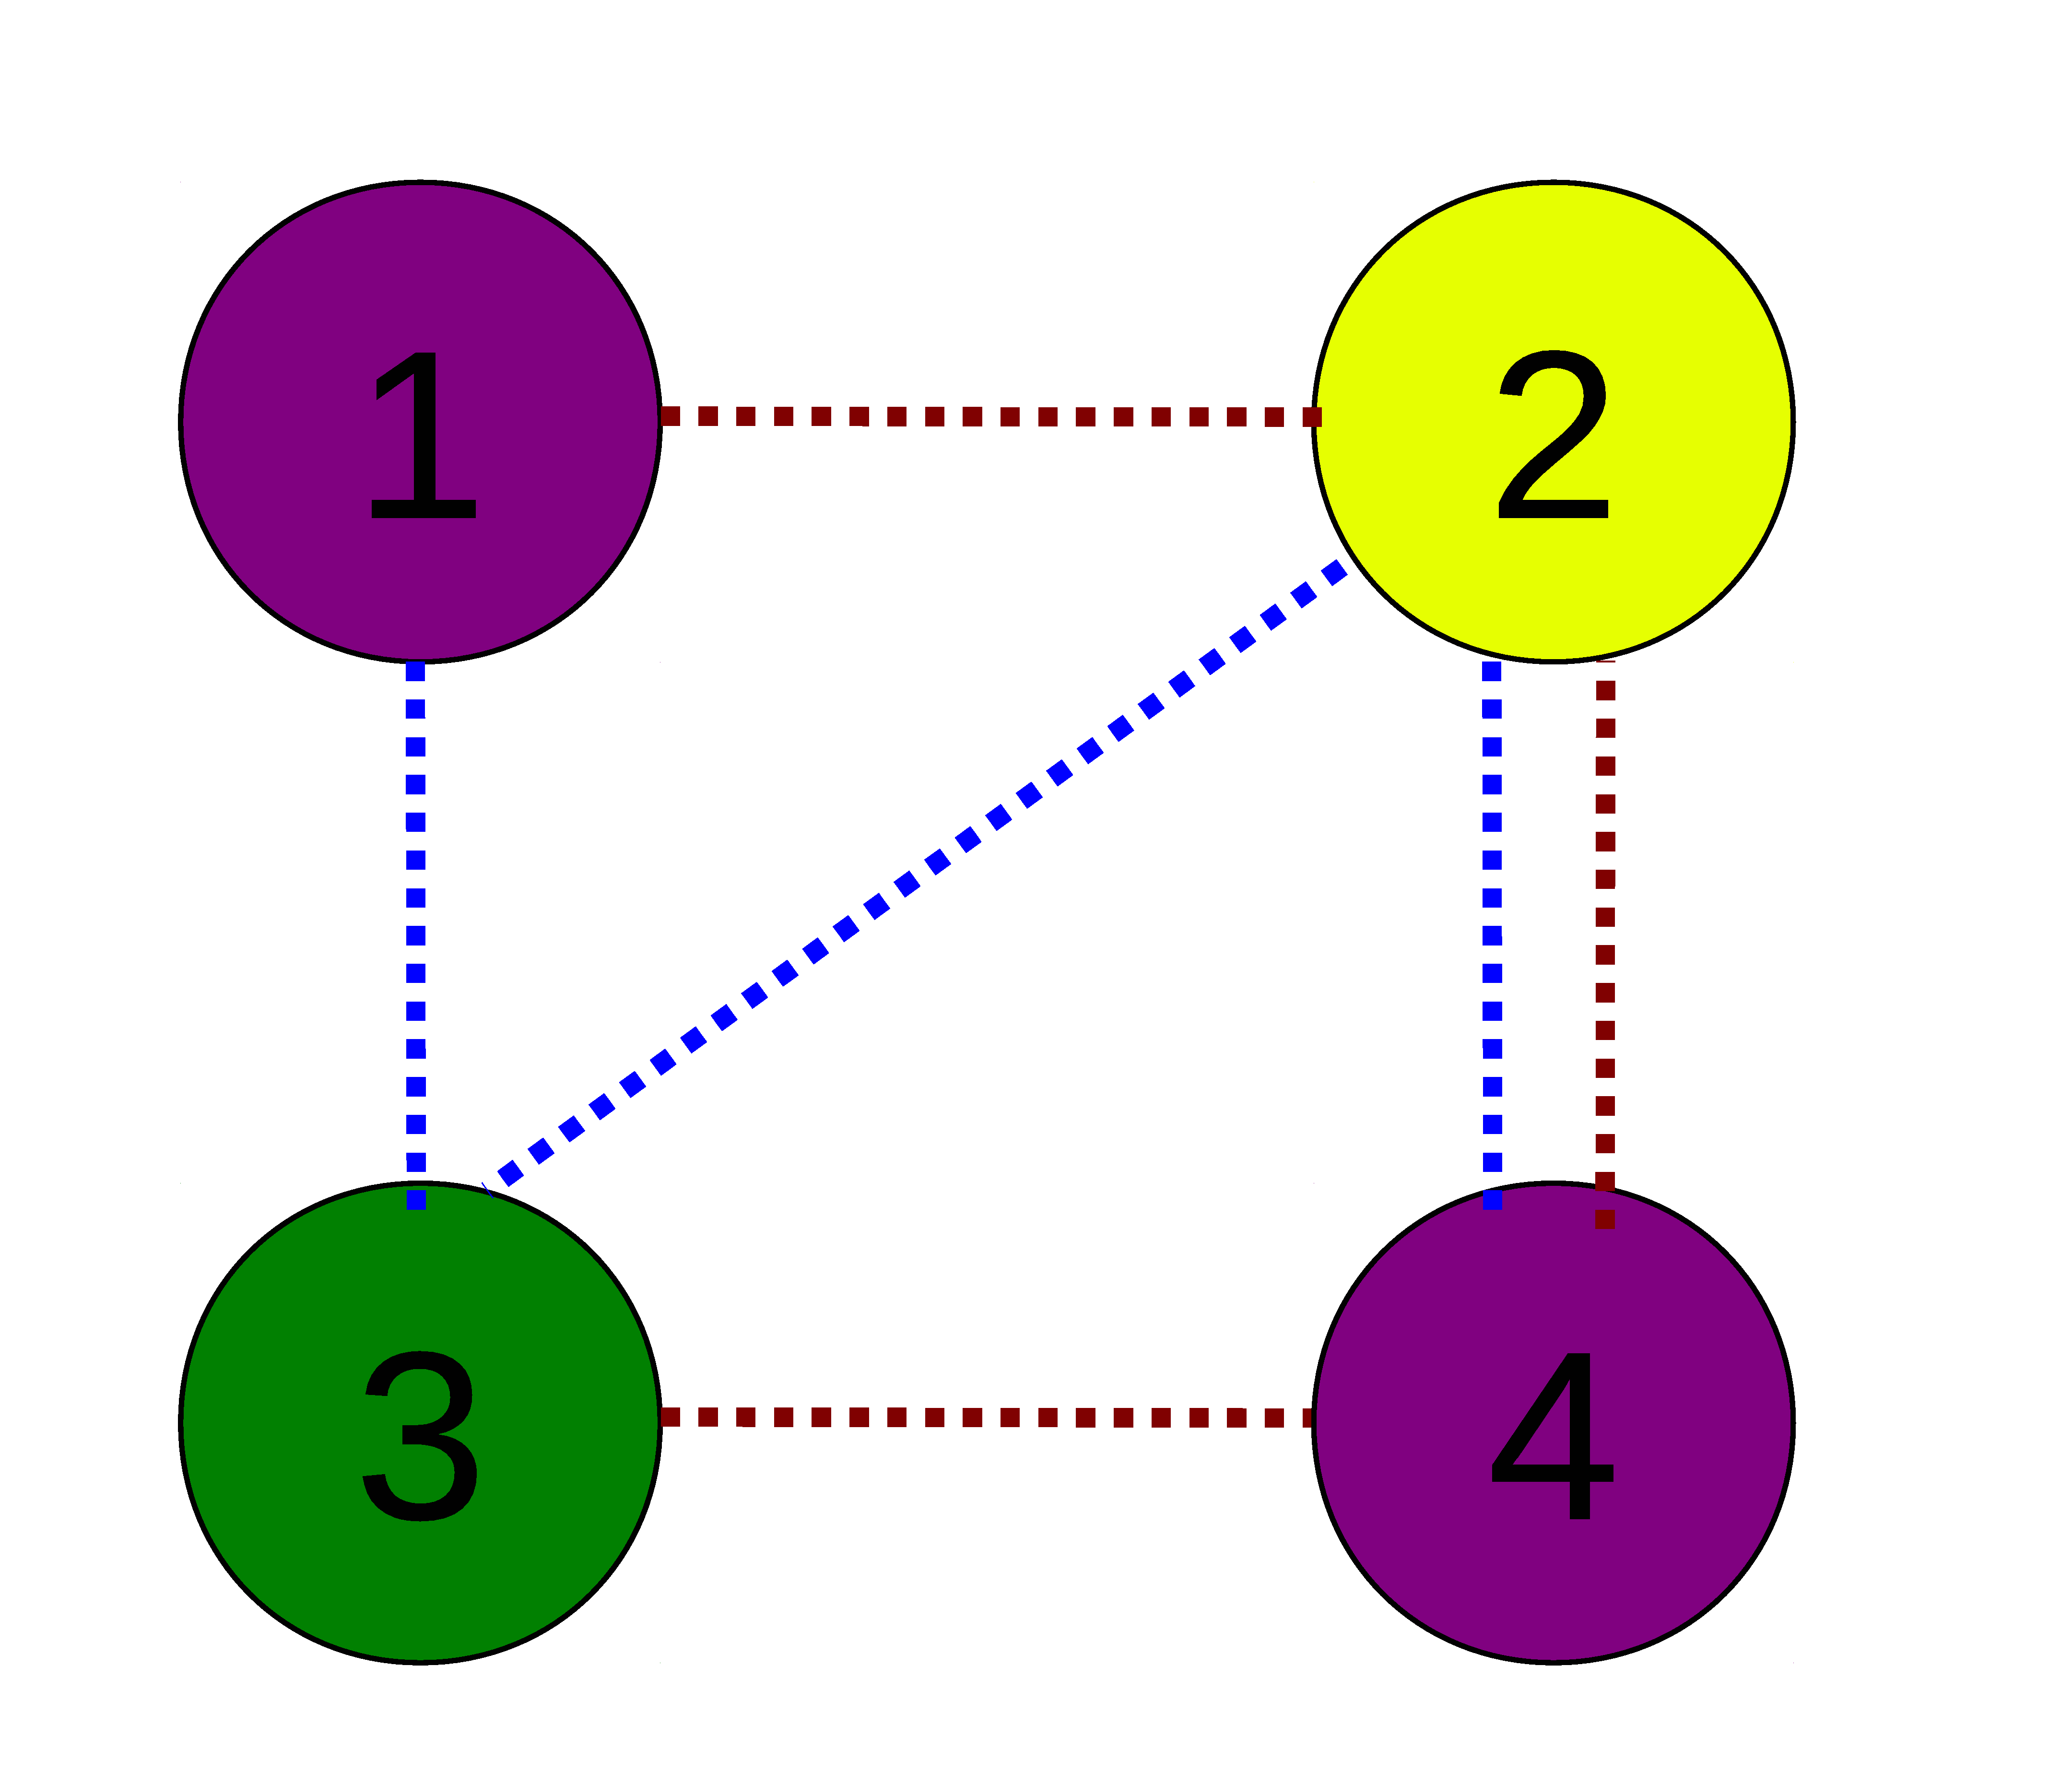
\epsfig{file=\fignet/ColoredMotif-SR.eps, width=.8\textwidth, clip=}
      \end{center}%$$
    \end{tabular}
    & 
    \hspace{-.5cm}
    \begin{tabular}{p{.45\textwidth}}
      \paragraph{Motif.} Connected component with prescribed topology
      \begin{center}%$$
      \epsfig{file=\fignet/version2.eps, width=0.25\textwidth}  
      %\epsfig{file=\fignet/version3.eps, width=0.3\textwidth}  
      %\epsfig{file=\fignet/version1.eps, width=0.3\textwidth} 
      \end{center}%$$
      ~\vspace{4cm}~ 
    \end{tabular}
  \end{tabular}
  }

%====================================================================
\subsection{Motif count}
\frame{\frametitle{Counting occurrences of topological motifs}
%==================================================================== 

  \paragraph{General principle.} Backtracking along the edges, ranked
  by decreasing degree + pruning.
  
  \bigskip\Pause
  \begin{tabular}{cc}
    \hspace{-.5cm}
    \begin{tabular}{p{.4\textwidth}}
      \paragraph{Pruning.} Given the occurrences of the red, brown and
      green vertices, $n(\mbf)$ is 
      $$
      {5 \choose 2} \times {4\choose 2}
      $$
      without further exploration.
    \end{tabular}
    & 
    \hspace{-.5cm}
    \begin{tabular}{p{.6\textwidth}}
      \epsfig{file=../FIGURES/Graph_08-SR.eps, scale=.2}
    \end{tabular}
  \end{tabular}

  \bigskip\Pause
  From $10^2$ to $10^3$ times faster than FanMod for motif count,
  about $10$ times faster for motif enumeration. (\refer{KGS11})
}
  
%==================================================================== 
\subsection{Null count distribution}
%====================================================================
\frame{\frametitle{Random graph null model}

  \paragraph{The null model} is supposed to generate random
  graphs $G_0$ 'similar' to the observed graphs $G_{\text{obs}}$.

  \bigskip\Pause
  \begin{tabular}{cc}
    \hspace{-.5cm}
    \begin{tabular}{p{.5\textwidth}}
      \paragraph{Metabolic network.}
      \begin{itemize}
      \item Coloured Erd�s = Erd�s edges + independent colors
      \end{itemize}
    \end{tabular}
    & 
    \hspace{-.5cm}
    \begin{tabular}{p{.5\textwidth}}
      \paragraph{Interaction network.}
      \begin{itemize}
      \item Stochastic block model
      \item Expected degree distribution
      \end{itemize}
    \end{tabular}
  \end{tabular} \\
  \ra Parameters are fitted to the observed graph $G_{\text{obs}}$.

  \bigskip\Pause
  \paragraph{Moments of the count.} Generic formulas for the mean and variance of the count moments can be derived for a large class of random graph
  models. \refer{PDK08} \refer{MSB06} \\
%   $$
%   \Esp[N(\mbf, G_0)], \qquad \qquad \Var[N(\mbf, G_0)].
%   $$
  The calculation of the variance requires to account for
  \emphase{overlaps between motif occurrences}.  
  }

%==================================================================== 
\subsection{(Approximate) distribution}
%====================================================================
\frame{\frametitle{(Approximate) distribution of the count}

  \begin{tabular}{cc}
    \hspace{-.5cm}
    \begin{tabular}{p{.45\textwidth}}
      \paragraph{(Approximate) distribution: } \\
      Polya-Aeppli = geometric Poisson
      $$
      N(\mbf, G_0) \approx \Pcal\Acal(\lambda, a),
      $$
      borrowed from sequences motifs.

      \bigskip\bigskip\Pause
      \paragraph{Parameters} $\lambda$ and $\alpha$ are fitted to the
      first two moments. 

      \bigskip
      \refer{SLS09} \\
      \refer{PDK08}

    \end{tabular}
    & 
    \hspace{-.5cm}
    \begin{tabular}{p{.5\textwidth}}
      \Pause\paragraph{Simulations} for coloured motifs \\~\\
      
      \epsfig{file=\fignet/SLS09-Fig4-BottomLeft.eps,
        width=.5\textwidth} 

      \textcolor{green}{Compound Poisson} provides a better fit than
      \textcolor{red}{Gaussian}. 
    \end{tabular}
  \end{tabular}

  }


%====================================================================
%====================================================================
\end{document}
%====================================================================
%====================================================================